\documentclass{beamer}

\usepackage{graphicx}

\titlepage
\title{Integrating a secondary constraint into SAIL to generate wheelcases that allow for more freedom} 
\author[Jan Kruska]{Jan Kruska}
\date[\today]{\today}


\begin{document}

\begin{frame}{}
	\titlepage
\end{frame}

\frame{\tableofcontents}

\section{Problem}
\frame{\frametitle{Problem}
	\begin{block}{Problem}
		The existing wheelcase inhibits the maximum steering angle of the wheels
	\end{block}
	\begin{itemize}
		\item It is simple to find solutions, that do not inhibit the maximum steering angle, e.g. make the wheelcase a box
		\item However such solutions are particularly bad in terms of aerodynamics
		\item It is much harder to find a solution with some degree of aerodynamic optimality, that does not inhibit the maximum steering angle
		\item The goal should be to generate solutions, which either don't inhibit the wheels, or at least don't do it as much as the current solution while still exhibiting some degree of aerodynamic optimality
	\end{itemize}
}
\section{Method}
\frame{\frametitle{SAIL}
SAIL is a surrogate assisted phenotypically divergent version of the genetic algorithm MAP-Elites.
\begin{itemize}
	\item Phenotypically divergent, it produces a diverse set of individuals, more specifically a map that is divided along phenotypic categories.
	\item Surrogate assisted, it makes use of a gaussian process as a surrogate to reduce the number of needed Evaluations of the real fitness function.
\end{itemize}

}
\frame{\frametitle{Categorization}
	\begin{itemize}
		\item MAP-Elites needs Categories to assign individuals their respective cells
		\item Currently the chosen Categories are:
		\begin{enumerate}
			\item Width of the velomobil
			\item x-Position of the widest Point\footnote{The velomobil is directed towards -X, so bigger values correspond to the widest point being further back}
		\end{enumerate}
	\end{itemize}
}
\frame{\frametitle{Soft Constraint vs. Hard Constraint}
	\begin{itemize}
		\item Two different solutions, which both violate the constraint, can still differ in terms of the severity of the violation
		\item The current wheelcase does violate the constraint, so at the beginning of the process no non-trivial solution, that fulfills the constraint, is known
		\item Because of those two considerations a soft constraint, seemed more useful for the problem at hand
	\end{itemize}
}

\frame{\frametitle{Modeling of the Constraint}
\begin{itemize}
	\item Due to the number of times the constraint has to be evaluated, the calculation needs to be reasonably fast
\end{itemize}
}

\frame{\frametitle{Steering Volume}
	The space needed by the wheel for all possible steering angles can be modeled as a volume:
	\begin{figure}
		\includegraphics[width=1\linewidth]{radausschlag00.png}
	\end{figure}
}

\frame{\frametitle{Constraint + Velomobil}
	This volume intersect with the current wheelcase 
	\begin{figure}
		\includegraphics[width=1\linewidth]{radausschlag_inclVelo01.png}
	\end{figure}
}

\frame{\frametitle{Constraint Volume}
	The Constraint can be calculated as the volume outside of the wheelcase, using mesh-difference operation
	\begin{figure}
		\includegraphics[width=1\linewidth]{difference00.png}
	\end{figure}
	This does not perfectly map to the real constraint, but it is stipulated, that the volume outside of the wheelcase is negatively correlated with the largest possible steering angle.
}

\section{First Results}
\frame{\frametitle{Setup}
	\begin{itemize}
		\item Two center points of a 3 by 4 grid used for deformation
		\item 250 OpenFoam simulations
		\item 1024 Generations for Acquisition
		\item 2048 Generations for final MAP-Elites
	\end{itemize}
}
\frame{\frametitle{Comparison non-constrained vs. constrained}
	\vspace*{\fill}
\begin{figure}
%	\centering
	
	\includegraphics[width=\linewidth]{short_boxplot_constraint}
\end{figure}
}

\frame{\frametitle{Comparison non-constrained vs. constrained}
	\vspace*{\fill}
	\begin{figure}
		%	\centering
		
		\includegraphics[width=\linewidth]{short_boxplot_fitness}
	\end{figure}
}


\frame{\frametitle{Fitness-maps}
	\begin{figure}
		\centering
		\includegraphics[height=.75\textheight]{short_map_fitness}
	\end{figure}
}

\frame{\frametitle{Top Left}
	\begin{figure}
		\centering
		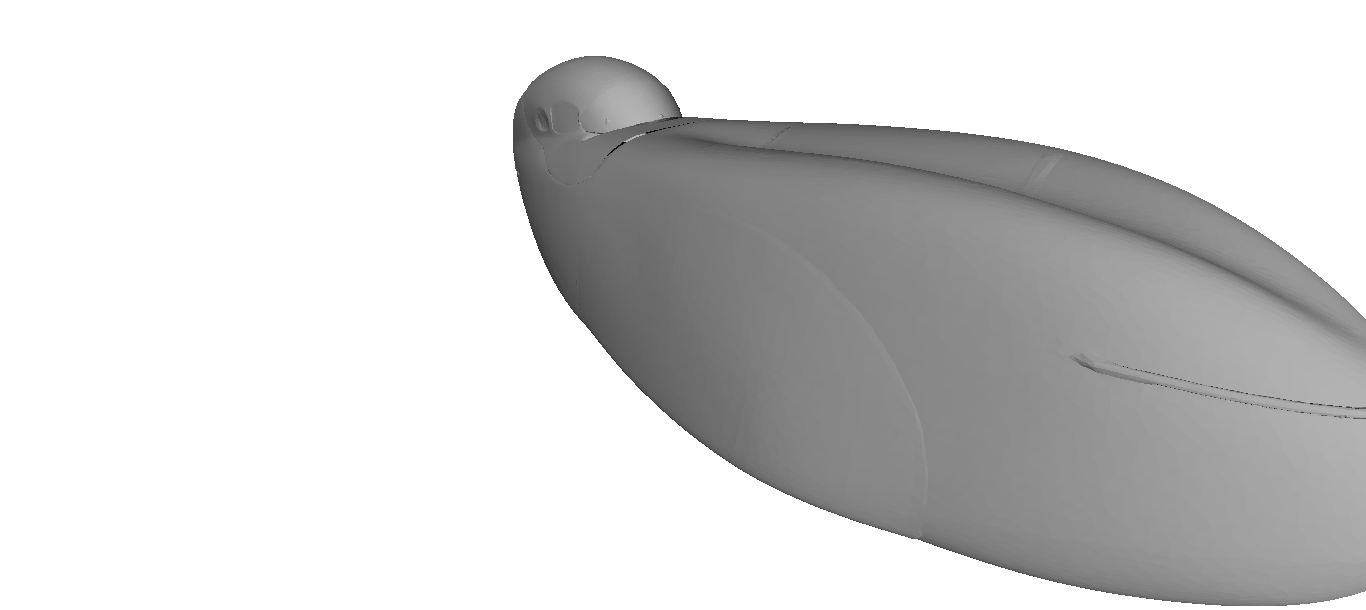
\includegraphics[width=\linewidth]{good00}
	\end{figure}
}

\frame{\frametitle{Bottom Right}
	\begin{figure}
		\centering
		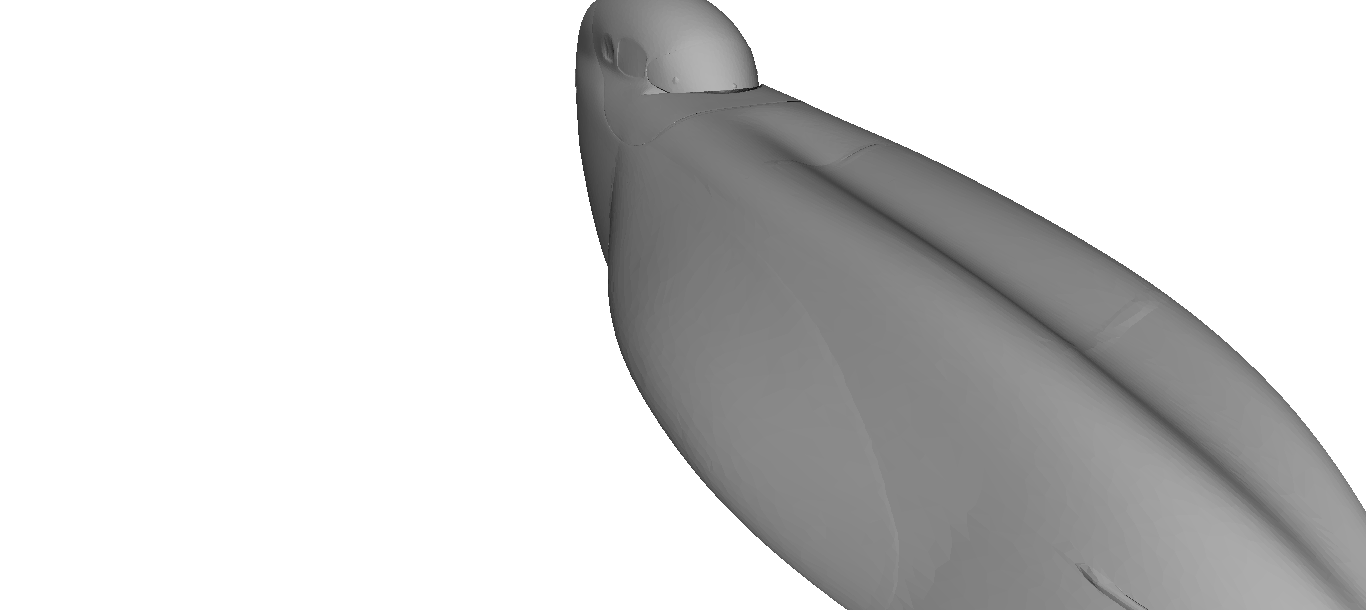
\includegraphics[width=\linewidth]{bad00}
	\end{figure}
}

\frame{\frametitle{Discussion}
	\begin{itemize}
		\item Fitness is worse, but this was expected
		\item The algorithm seems to work towards fulfilling the constraint
	\end{itemize}
}
\section{Future experiments}
\frame{\frametitle{Future changes}
\begin{itemize}
	\item Change FFD-parameters, to facilitate more degrees of freedom
	\item Longer rund, more generations \& more OpenFoam Evaluations
\end{itemize}
}


\end{document}
